\documentclass{standalone}
\usepackage{tikz}
\begin{document}
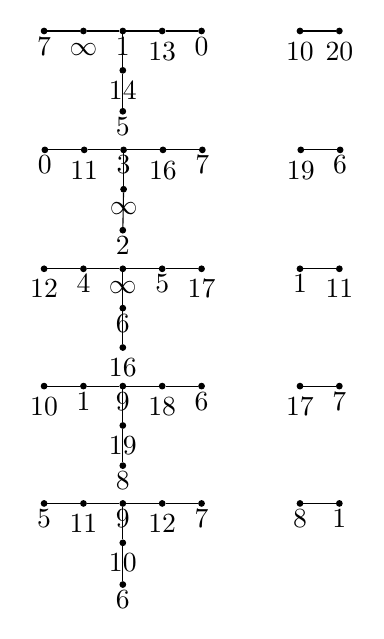
\begin{tikzpicture}[every node/.style={draw, circle, fill=black, minimum size=2pt, inner sep=0pt}]
\node[fill=black, label=below:{\color{black}$7$}] (G1N7) at (4.00,7.51) {};
\node[fill=black, label=below:{\color{black}$\infty$}] (G1Ninf) at (4.50,7.51) {};
\node[fill=black, label=below:{\color{black}$1$}] (G1N1) at (5.00,7.51) {};
\node[fill=black, label=below:{\color{black}$13$}] (G1N13) at (5.50,7.51) {};
\node[fill=black, label=below:{\color{black}$0$}] (G1N0) at (6.00,7.51) {};
\node[fill=black, label=below:{\color{black}$14$}] (G1N14) at (5.00,7.01) {};
\node[fill=black, label=below:{\color{black}$5$}] (G1N5) at (5.00,6.49) {};
\node[fill=black, label=below:{\color{black}$10$}] (G1N10) at (7.25,7.51) {};
\node[fill=black, label=below:{\color{black}$20$}] (G1N20) at (7.75,7.51) {};
\draw (G1N7) -- (G1Ninf);
\draw (G1Ninf) -- (G1N1);
\draw (G1N1) -- (G1N13);
\draw (G1N1) -- (G1N14);
\draw (G1N13) -- (G1N0);
\draw (G1N14) -- (G1N5);
\draw (G1N10) -- (G1N20);
\node[fill=black, label=below:{\color{black}$0$}] (G2N0) at (4.01,6.00) {};
\node[fill=black, label=below:{\color{black}$11$}] (G2N11) at (4.51,6.00) {};
\node[fill=black, label=below:{\color{black}$3$}] (G2N3) at (5.01,6.00) {};
\node[fill=black, label=below:{\color{black}$16$}] (G2N16) at (5.51,6.00) {};
\node[fill=black, label=below:{\color{black}$7$}] (G2N7) at (6.01,6.00) {};
\node[fill=black, label=below:{\color{black}$\infty$}] (G2Ninf) at (5.01,5.50) {};
\node[fill=black, label=below:{\color{black}$2$}] (G2N2) at (5.00,4.98) {};
\node[fill=black, label=below:{\color{black}$19$}] (G2N19) at (7.26,6.00) {};
\node[fill=black, label=below:{\color{black}$6$}] (G2N6) at (7.76,6.00) {};
\draw (G2N0) -- (G2N11);
\draw (G2N11) -- (G2N3);
\draw (G2N3) -- (G2N16);
\draw (G2N3) -- (G2Ninf);
\draw (G2N16) -- (G2N7);
\draw (G2Ninf) -- (G2N2);
\draw (G2N6) -- (G2N19);
\node[fill=black, label=below:{\color{black}$12$}] (G3N12) at (4.00,4.49) {};
\node[fill=black, label=below:{\color{black}$4$}] (G3N4) at (4.50,4.49) {};
\node[fill=black, label=below:{\color{black}$\infty$}] (G3Ninf) at (5.00,4.49) {};
\node[fill=black, label=below:{\color{black}$5$}] (G3N5) at (5.50,4.49) {};
\node[fill=black, label=below:{\color{black}$17$}] (G3N17) at (6.00,4.49) {};
\node[fill=black, label=below:{\color{black}$6$}] (G3N6) at (5.00,3.99) {};
\node[fill=black, label=below:{\color{black}$16$}] (G3N16) at (5.00,3.49) {};
\node[fill=black, label=below:{\color{black}$1$}] (G3N1) at (7.25,4.49) {};
\node[fill=black, label=below:{\color{black}$11$}] (G3N11) at (7.75,4.49) {};
\draw (G3N12) -- (G3N4);
\draw (G3N4) -- (G3Ninf);
\draw (G3Ninf) -- (G3N5);
\draw (G3Ninf) -- (G3N6);
\draw (G3N5) -- (G3N17);
\draw (G3N6) -- (G3N16);
\draw (G3N1) -- (G3N11);
\node[fill=black, label=below:{\color{black}$10$}] (G4N10) at (4.00,3.00) {};
\node[fill=black, label=below:{\color{black}$1$}] (G4N1) at (4.50,3.00) {};
\node[fill=black, label=below:{\color{black}$9$}] (G4N9) at (5.00,3.00) {};
\node[fill=black, label=below:{\color{black}$18$}] (G4N18) at (5.50,3.00) {};
\node[fill=black, label=below:{\color{black}$6$}] (G4N6) at (6.00,3.00) {};
\node[fill=black, label=below:{\color{black}$19$}] (G4N19) at (5.00,2.50) {};
\node[fill=black, label=below:{\color{black}$8$}] (G4N8) at (5.00,1.99) {};
\node[fill=black, label=below:{\color{black}$17$}] (G4N17) at (7.25,3.00) {};
\node[fill=black, label=below:{\color{black}$7$}] (G4N7) at (7.75,3.00) {};
\draw (G4N10) -- (G4N1);
\draw (G4N1) -- (G4N9);
\draw (G4N9) -- (G4N18);
\draw (G4N9) -- (G4N19);
\draw (G4N18) -- (G4N6);
\draw (G4N19) -- (G4N8);
\draw (G4N7) -- (G4N17);
\node[fill=black, label=below:{\color{black}$5$}] (G5N5) at (4.00,1.51) {};
\node[fill=black, label=below:{\color{black}$11$}] (G5N11) at (4.50,1.51) {};
\node[fill=black, label=below:{\color{black}$9$}] (G5N9) at (5.00,1.51) {};
\node[fill=black, label=below:{\color{black}$12$}] (G5N12) at (5.50,1.51) {};
\node[fill=black, label=below:{\color{black}$7$}] (G5N7) at (6.00,1.51) {};
\node[fill=black, label=below:{\color{black}$10$}] (G5N10) at (5.00,1.01) {};
\node[fill=black, label=below:{\color{black}$6$}] (G5N6) at (5.00,0.48) {};
\node[fill=black, label=below:{\color{black}$8$}] (G5N8) at (7.25,1.51) {};
\node[fill=black, label=below:{\color{black}$1$}] (G5N1) at (7.75,1.51) {};
\draw (G5N5) -- (G5N11);
\draw (G5N11) -- (G5N9);
\draw (G5N9) -- (G5N12);
\draw (G5N9) -- (G5N10);
\draw (G5N12) -- (G5N7);
\draw (G5N10) -- (G5N6);
\draw (G5N1) -- (G5N8);
\end{tikzpicture}
\end{document}
